%% Template file for seminar papers
%% based on bare_conf.tex V 1.3 (2007/01/11) by Michael Shell (http://www.michaelshell.org/)
% Do not adjust lengths that control margins, column widths, etc.
% Do not use packages that alter fonts (such as pslatex).         

%% TODO: alle "?!" weg?

\documentclass[conference]{IEEEtran}


\usepackage[utf8]{inputenc} % Kodierung
\usepackage[ngerman]{babel} % Sprache
\usepackage{makeidx}  % allows for indexgeneration

\usepackage{math}
\usepackage{amsfonts}
\usepackage{graphicx}
\usepackage{subcaption}
\usepackage{url}

% correct bad hyphenation here
%\hyphenation{op-tical net-works semi-conduc-tor}


\begin{document}
%
% paper title
% can use linebreaks \\ within to get better formatting as desired
\title{Bilaterale Filter und Diffusionsfilter}


\author{\IEEEauthorblockN{Markus Braunwarth}
\IEEEauthorblockA{
E-Mail: {\tt mbraunwarth@uni-koblenz.de}, Matrikelnummer: 215200130 \\
Proseminar Bildverarbeitung, Wintersemester 2018/19, Universität Koblenz-Landau
}}


% make the title area
\maketitle


\begin{abstract}

% erstsen Satz ergänzen (zu knapp)
Im Folgenden sollen Bilaterale Filter und die anisotropische Diffusion betrachtet werden. Der Schwerpunkt liegt hierbei auf Methoden zur Glättung von Grauwert- und Farbbildern wobei Kanten nicht verschmiert werden sollen, wie es bei vielen Filtern der Fall ist. Dazu werden zuerst Glättungsfilter im allgemeinen betrachtet und die Probleme, welche Kanten beim glätten von Bildern verursachen können. 

\end{abstract}

% For peerreview papers, this IEEEtran command inserts a page break and
% creates the second title. It will be ignored for other modes.
\IEEEpeerreviewmaketitle



\section{Einleitung}

In einer Vielzahl von Anwendungen der Datenverarbeitung ist es oft wichtig, Rauschen in Bildern zu verringern ohne den Umriss von Objekten zu verändern. Methoden wie der Gauß-Filter glätten Bilder zwar, jedoch werden mit dem Rauschen auch Kanten verschmiert. Unter der Verwendung Bilateraler Filter \cite{tomasi1998bilateral} und bestimmter Diffusionsfilter \cite{perona1990scale} lassen sich Bilder glätten ohne diese Kanten zu verschmieren.

In dieser Ausarbeitung werden zunächst die Unterschiede linearer und nichtlinearer Filter erläutert sowie jene zwischen \textit{domain} und \textit{range} Filtern. Zur visuellen Darstellung des Problems folgt ein Vergleich der Kantenerhaltenden Glättung durch Bilaterale Filterung zu Glättungsfiltern, welche Kanten verschmieren. Darüber hinaus wird die bilaterale Filterung sowie der Perona-Malik-Filter näher beleuchtet. Ergänzend werden die Filtermethoden sowohl in Grauwert- als auch in Farbbildern betrachtet.


%% TODO: FILTERMASKE vs FALTUNGSKERN vs KERNEL??%%

\section{Glättungsfilter}

%% Hier bitte Kern und Faltung einführen
Glättungsfilter sind in der Regel Funktionen (bzw. Matrizen), welche mit dem Bild gefaltet werden und so Verunreinigungen (Rauschen) aus dem Bild entfernen sollen.
Filter können in verschiedene Arten unterteilt werden, von denen im folgenden die Linearität näher beleuchtet und der Unterschied von \textit{domain} und \textit{range} Filtern geklärt wird.

\subsection{Linearität von Filtern}



\subsection{Domain vs. Range Filter}

% richtiger zitierstil?
vgl \cite{burger2009principles}
Ein \textit{domain} Filter kodiert den Abstand der Nachbarpixel in das Ergebnis. Je weiter ein Pixel vom Mittelpunkt des Faltungskerns entfernt ist, desto weniger fließt sein Wert in das Ergebnis der Faltung mit ein. Die Gewichte der Filtermaske sind also abhängig vom relativen(?!) Abstand zu ihrem Mittelpunkt.
Die Einträge eines Faltungskerns von \textit{range} Filtern hingegen sind nicht abhängig von der Entfernung eines Nachbarpixels zum Mittelpunkt des Kerns, sondern von seiner Ähnlichkeit zu diesem, also dem Abstand Abstand ihrer Farbwerte (weiterhin als Intensität bezeichnet). So kann verhindert werden, dass die Filteroperation Kanten verschmiert.

\subsection{Probleme mit Kanten}
%% Gauss filter?

\section{Kantenerhaltende Filter}

\subsection{Bilaterale Filter}

Das Konzept des bilateralen Filterns wurde erstmals in \cite{tomasi1998bilateral} von Tomasi und Manduchi eingeführt. 
Es berücksichtigt sowohl den räumlichen Abstand der Pixel als auch den Abstand ihrer Intensitäten. Je näher die Intensitäten aneinander liegen, desto stärker beeinflusst der Pixel das Endergebnis. Sehr unterschiedliche Intensitäten hingegen sorgen dafür, dass dieser Pixel das Endergebnis weniger beeinflusst. 
Da Pixel an Kanten meist hohen Kontrast, also starke Intensitätsschwankungen aufweisen, kann so gewährleistet werden, dass Pixel jenseits einer Kante weniger stark ins Gewicht fallen.
Formal ist der Bilaterale Filter wie folgt definiert:

\begin{eqnarray}
\bm{I'}(\bm u) = \frac {1}{W} \sum_{i = -K}^{K} \sum_{j = -K}^{K} 
\bm I(u_1 + i, u_2 + j) 
\cdot H_d(i, j) \\
\cdot H_r(\bm I(u_1+i, u_2+j) - \bm I(u_1, u_2)).
\end{eqnarray}

Hierbei ist $\bm{I'}$ das resultierende gefilterte Bild, $\bm{I}$ das zu filternde Bild und $\bm{u}$ ein zweidimensionaler Ortsvektor welcher in $\bm I(\bm u)$ einen Bildpixel repräsentiert. Die Formel verkörpert eine Faltung mit einem Kernel der Größe $K$, der \textit{domain} Gewichtsfunktion

\begin{equation}
H_d(m, n) = 
	\exp \left( -
		\frac{ (m^2 + n^2) } {2 \sigma_d^2} 
	\right),
\end{equation}

welche den räumlichen Abstand zweier Pixel ausdrückt und analog der \textit{range} Gewichtsfunktion

\begin{equation}
H_r(x) = 
	\exp \left( -
		\frac{ x^2 } {2 \sigma_r^2} 
	\right),
\end{equation}

welche deren Intensitätsabstand ausdrückt, wobei $H_r$ die Differenz der Pixel als Parameter erwartet. Der Ausdruck $\frac 1{W}$ normiert das Ergebnis mit der Summe der Gewichte:

\begin{equation}
W_{u,v} = \sum_{i = -K}^{K} \sum_{j = -K}^{K} H_d(i,j) \cdot H_r(\bm I(u_1+i, u_2+j) - \bm I(u_1, u_2)).
\end{equation}


\subsection{Anisotropische Diffusion}

Beruhend auf dem physikalischen Konzept der Diffusion, zum Modellieren von Partikelverteilungen in einem Medium, werden Diffusionsgleichungen in der Bildverarbeitung zum Glätten von Bildern eingesetzt. Dabei ist zu unterscheiden zwischen isotropischer und anisotropischer Diffusion. Bei näherer Betrachtung der isotropischen Diffusion fällt auf, dass sie die selben Ergebnisse liefert wie der Gaus-Filter (vgl. \cite{burger2009principles}, S. 145) und damit nicht zur kantenerhaltenden Glättung dient. Perona und Malik erarbeiteten nun in \cite{perona1990scale} die von ihnen als anisotropische Diffusion bezeichnete Filtermethode, welchein der Bildverarbeitung noch heute in Gebrauch ist und weiter erforscht wird.
Der Perona-Malik-Filter genannte Diffusionsfilter ist tatsächlich isotropisch ist und nur anisotropisch erscheint wird er in der Literatur meist als anisotropisch aufgefasst (vgl. \cite{weickert1998anisotropic}, S. 15).

Der Perona-Malik-Filter bedient sich eines iterativen Schemas, wodurch die Ergebnisse eines Filterdurchlaufs den nächsten beeinflussen. Das Originalbild $\bm I$ wird daher als $\bm I^{(0)}$ bezeichnet, das Ergebnisbild des $n$-ten Durchlaufes ist durch $I^{(n)}$ gegeben. Formal ist der $n$-te Durchlauf des Perona-Malik-Filters wie folgt:
% summe erklären -> 0 bis 3 <= 4 nachbarn

\begin{equation}
\bm I^{(n)}(\bm u) = 
	\bm I^{(n-1)}(\bm u) + \alpha 
	\cdot \sum_{i=0}^3 g(|\delta_i (\bm I^{(n-1)}, \bm u)|) 
	\cdot \delta_i (\bm I^{(n-1)}, \bm u)
\end{equation}

Wobei $\delta (\bm I, \bm u) = \bm I(\bm u + \bm d_i) - \bm I(\bm u)$ die Differenz des Pixels $\bm I(\bm u)$ und seinem $i$-ten Nachbarn angibt.
In der Formel wird das bereits erwähnte iterative Verhalten des Filters deutlich. $0 < \alpha \leq 1$ ist ein Konstanter Faktor welcher bestimmt, wie stark das Ergebnis des momentanen Durchlaufs dem vorherigen beeinflusst.

$g(d): \mathbb R \rightarrow [0,1]$ ist die sogenannte \textit{conductivity function}. Sie liefert hohe Werte in homogenen Regionen und niedrige Werte in der Nähe von Kanten. So werden die Nachbarpixel von $\bm u$ gewichtet und Pixeln nahe (oder in) einer Kante werden weniger berücksichtigt als Nachbarpixel in homogenen Flächen.
Für die \textit{conductivity function} gibt es bereits häufig verwendete Vertreter welche jeweils selbst ein bestimmtes Verhalten zur Diffusion beitragen wie zum Beispiel kontrastreiche Kanten zu präferieren \cite{burger2009principles}. Um einige zu nennen:

\begin{equation}
g_1(d) = \exp {- \left( \frac{d}{\kappa} \right)^2}
\qquad
g_2(d) = \frac{1}{1+((d/\kappa)^2}.
\end{equation}

Ihre jeweiligen Eigenschaften werden in dieser Ausarbeitung jedoch nicht weiter beleuchtet.

\section{Fazit}

\begin{figure}
  \begin{subfigure}[b]{0.4\textwidth}
    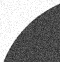
\includegraphics[width=\linewidth]{img/cut/noisy_circle.png}
    \caption{Verrauschtes Bild}
    \label{fig:1}
  \end{subfigure}
  %
  \begin{subfigure}[b]{0.4\textwidth}
    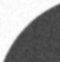
\includegraphics[width=\linewidth]{img/cut/gaussian_filtered.png}
    \caption{Gauß-Filter}
    \label{fig:2}
  \end{subfigure}
  %
  \begin{subfigure}[b]{0.4\textwidth}
    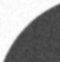
\includegraphics[width=\linewidth]{img/cut/gaussian_filtered.png}
    \caption{Anisotropische Diffusion}
    \label{fig:3}
  \end{subfigure}
  %
  \begin{subfigure}[b]{0.4\textwidth}
    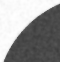
\includegraphics[width=\linewidth]{img/cut/bilateral_filtered.png}
    \caption{Bilateral Filter}
    \label{fig:4}
  \end{subfigure}
\end{figure}


% Bib aktualisieren: F6 -> F6 -> F11 -> F6
\bibliographystyle{alpha}
\bibliography{literatur}

\end{document}
